\subsection{Electrostatics \& Magnetostatics}

\begin{frame}{Electrostatics \& Magnetostatics}
    \begin{columns}
        \column{0.5\textwidth}
        \vspace{-7mm}
        \begin{center}
            \textcolor{BlueDefault}{Electrostatics}
        \end{center}
        
        \begin{itemize}
            \item \( \mathbf{j} \approx 0\) and \( \mathbf{B} \approx 0\).
            \item \( \nabla \cdot \mathbf{D} = \rho \) and \( \nabla \times \mathbf{E} = 0 \).
            \item \( \phi = \dfrac{1}{4\pi\varepsilon_0} \int \dfrac{\rho}{|\mathbf{r}-\mathbf{r}'|} \mathrm{d}^3\mathbf{r}' \).
        \end{itemize}

        \vspace{2mm}
        \begin{figure}[!htb]
        \centering
        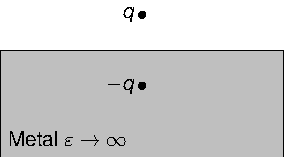
\includegraphics[width=\textwidth]{Figures/Image_method.pdf}
        \caption{Electrostatics problem.}
        \label{Image_method}
        \end{figure}

        \column{0.5\textwidth}
        \vspace{-7mm}

        \begin{center}
            \textcolor{BlueDefault}{Magnetostatics}
        \end{center}
        
        \begin{itemize}
            \item \( \mathbf{j} = \text{const} \) and \( \mathbf{B} = \text{const} \).
            \item \( \nabla \cdot \mathbf{B} = 0 \) and \( \nabla \times \mathbf{H} = \mathbf{j} \).
            \item \( \mathbf{A}(\mathbf{r}) = \dfrac{\mu_{0}}{4\pi} \int{ \dfrac{\mathbf{J(\mathbf{r}')} } {|\mathbf{r}-\mathbf{r}'|} \mathrm{d}^3\mathbf{r}'} \).
        \end{itemize}
        
        \vspace{-2mm}
        \begin{figure}[!htb]
        \centering
        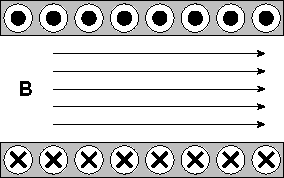
\includegraphics[width=\textwidth]{Figures/Soleloid.pdf}
        \caption{Magnetostatics problem.}
        \label{Soleloid}
        \end{figure}
    \end{columns}
\end{frame}